\documentclass{article}

\usepackage{graphicx}
\usepackage{tikz}
\usepackage{tikzsymbols}
\usetikzlibrary{calc,patterns,shapes.geometric}
\pagestyle{empty}
\usepackage[margin=0pt]{geometry}
\geometry{papersize={14in,12in}}

\def\centerarc[#1](#2)(#3:#4:#5){\draw[#1] ($(#2)+({#5*cos(#3)},{#5*sin(#3)})$) arc (#3:#4:#5);}

\begin{document}
	\begin{figure}
		\centering
		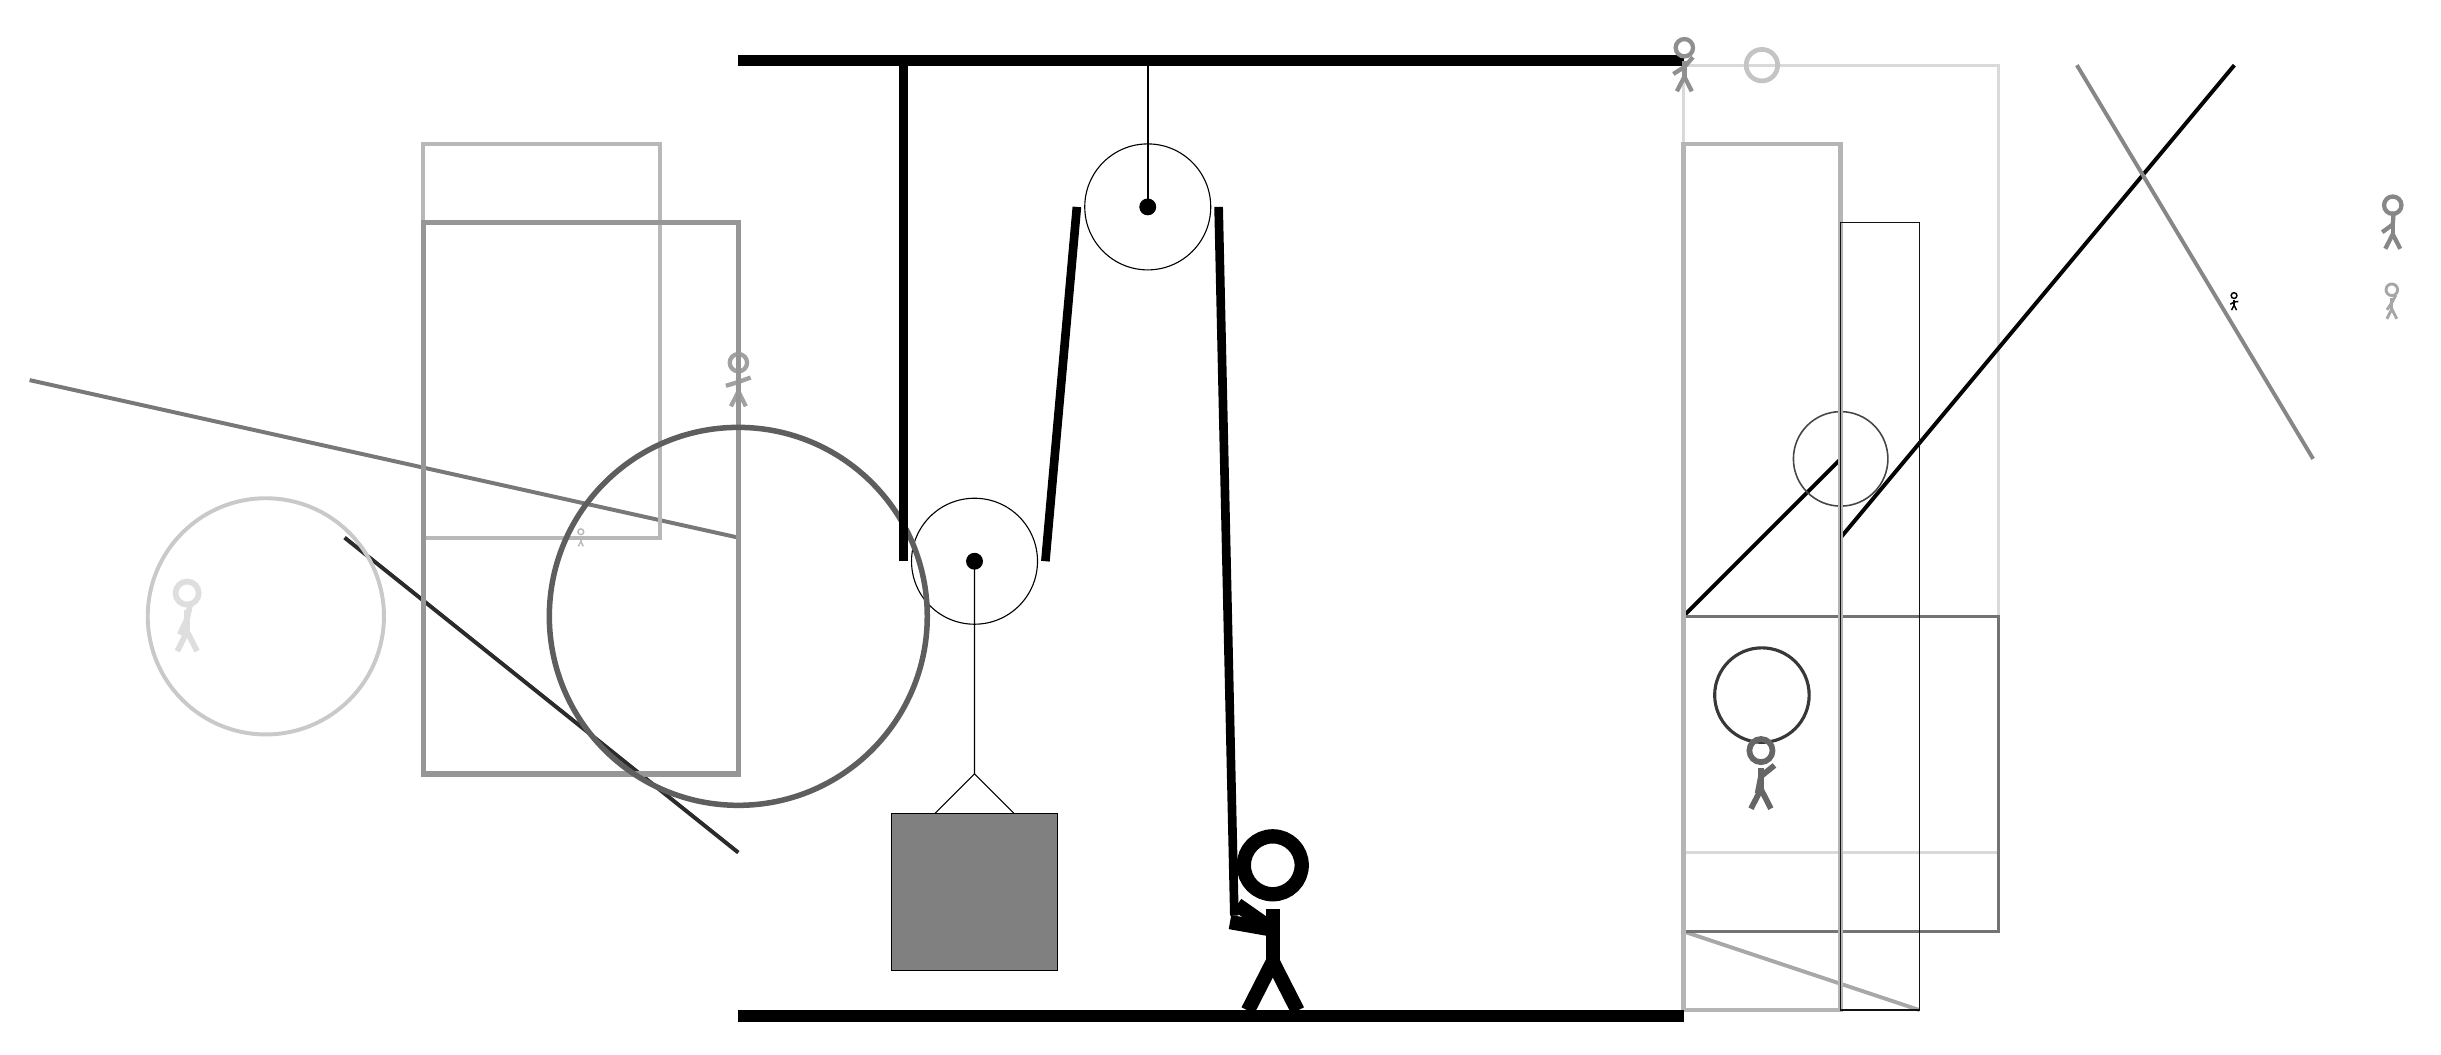
\begin{tikzpicture}
			%%%%% START %%%%%
			
			\draw[fill=black] (-2, 9) rectangle (10, 9.125);
			
			\draw (3.2, 7.2) circle (0.8);
			\draw[fill=black] (3.2, 7.2) circle (0.1);
			\draw[thick] (3.2, 7.2) -- (3.2, 9);
			
			\draw (1, 2.7) circle (0.8);
			\draw[fill=black] (1, 2.7) circle (0.1);
			
			\draw [line width=0.4mm, color=black!78](11, 1) circle (0.6);
			
			\draw[line width=0.5mm, color=black!83](-7, 3) -- (-2, -1);
			\draw[line width=0.5mm, color=black!100](12, 4) -- (10, 2);
			\draw[line width=0.5mm, color=black!27] (-3, 4) rectangle (-3, 4);
			
			\draw[line width=0.4mm, color=black!15] (10, -1) rectangle (14, 9);
			\node[line width=0.5mm, color=black!60] at (11, 0) {\Strichmaxerl[4][79][39]};
			
			\draw[line width=0.5mm, color=black!34](10, -2) -- (13, -3);
			\draw[line width=0.4mm, color=black!55] (10, -2) rectangle (14, 2);
			\node[line width=0.6mm, color=black!37] at (-2, 5) {\Strichmaxerl[3][17][20]};
			\draw [line width=0.6mm, color=black!23](11, 9) circle (0.2);
			
			\node[line width=0.6mm, color=black!44] at (10, 9) {\Strichmaxerl[3][32][49]};
			\node[line width=0.6mm, color=black!28] at (-4, 3) {\Strichmaxerl[1][4][11]};
			\draw[line width=0.5mm, color=black!98](12, 3) -- (17, 9);
			
			\draw [line width=0.2mm, color=black!73](12, 4) circle (0.6);
			\draw[line width=0.5mm, color=black!53](-2, 3) -- (-11, 5);
			\node[line width=0.5mm, color=black!35] at (19, 6) {\Strichmaxerl[2][56][62]};
			\draw[line width=0.5mm, color=black!28] (-3, 8) rectangle (-6, 3);
			
			\node[line width=0.4mm, color=black!47] at (19, 7) {\Strichmaxerl[3][36][86]};
			\draw[line width=0.3mm, color=black!24] (10, 1) rectangle (10, 4);
			
			\draw[line width=0.5mm, color=black!47](15, 9) -- (18, 4);
			\node[line width=0.4mm, color=black!100] at (17, 6) {\Strichmaxerl[1][31][7]};
			
			\draw[line width=0.6mm, color=black!29] (12, -3) rectangle (10, 8);
			
			\draw[line width=0.7mm, color=black!41] (-2, 0) rectangle (-6, 7);
			\draw [line width=0.7mm, color=black!63](-2, 2) circle (2.4);
			\node[line width=0.2mm, color=black!13] at (-9, 2) {\Strichmaxerl[4][65][78]};
			
			\draw[line width=0.2mm, color=black!93] (12, -3) rectangle (13, 7);
			\draw [line width=0.5mm, color=black!21](-8, 2) circle (1.5);
			
			\draw (1, 2.7) -- (1, 0) -- (0.5, -0.5);
			\draw (1, 0) -- (1.5, -0.5);
			\draw[fill=black!50] (-0.05, -0.5) rectangle (2.05, -2.5);
			
			\draw[line width=1.1mm] (0.1, 9) -- (0.1, 2.7);
			\centerarc[line width=1.1mm](1, 2.7)(180:360:0.9);
			\draw[line width=1.1mm](1.9, 2.7) -- (2.3, 7.2);
			\centerarc[line width=1.1mm](3.2, 7.2)(0:180:0.9);
			\draw[line width=1.1mm](4.1, 7.2) -- (4.3, -1.8);
			
			\node at (4.7, -1.9) {\Strichmaxerl[10][-35][170]};
			
			\draw[fill=black] (-2, -3) rectangle (10, -3.15);
			
			%%%%% END %%%%%
		\end{tikzpicture}
	\end{figure}	
\end{document}